\documentclass[a4paper, 12pt]{report}
\usepackage{cmap}
\usepackage{amssymb}
\usepackage{amsmath}
\usepackage{graphicx}
\usepackage{amsthm}
\usepackage{upgreek}
\usepackage{listings}
\usepackage{setspace}
\usepackage[T2A]{fontenc}
\usepackage[utf8]{inputenc}
\usepackage[normalem]{ulem}
\usepackage{mathtext} % русские буквы в формулах
\usepackage[left=2cm,right=2cm, top=2cm,bottom=2cm,bindingoffset=0cm]{geometry}
\usepackage[english,russian]{babel}
\usepackage[unicode]{hyperref}
\usepackage{pythonhighlight}
\newcommand\Norm[1]{\left\| #1 \right\|}
\newcommand{\dif}{\mathrm{d}}
\newcommand{\Rm}{\mathbb{R}}
\newcommand{\Cm}{\mathbb{C}}
\newcommand{\Z}{\mathbb{Z}}
\newcommand{\I}{\mathbb{I}}
\newcommand{\N}{\mathbb{N}}
\newcommand{\rank}{\operatorname{rank}}
\newcommand{\Ra}{\Rightarrow}
\newcommand{\ra}{\rightarrow}
\newcommand{\FI}{\Phi}
\newcommand{\Sp}{\text{Sp}}
\renewcommand{\leq}{\leqslant}
\renewcommand{\geq}{\geqslant}
\renewcommand{\alpha}{\upalpha}
\renewcommand{\beta}{\upbeta}
\renewcommand{\gamma}{\upgamma}
\renewcommand{\delta}{\updelta}
\renewcommand{\varphi}{\upvarphi}
\renewcommand{\tau}{\uptau}
\renewcommand{\lambda}{\uplambda}
\renewcommand{\psi}{\uppsi}
\renewcommand{\mu}{\upmu}
\renewcommand{\omega}{\upomega}
\renewcommand{\d}{\partial}
\renewcommand{\xi}{\upxi}
\renewcommand{\epsilon}{\upvarepsilon}
\newtheorem*{theorem}{Теорема}
\newtheorem*{cor}{Следствие}
\newtheorem*{lem}{Лемма}
	% Переоформление некоторых стандартных названий


\begin{document}
\renewcommand{\chaptername}{Контрольная самостоятельная работа}
\def\contentsname{Содержание}
	
	% Оформление титульного листа
	\begin{titlepage}
		\begin{center}
			\textsc{МИНИСТЕРСТВО ОБРАЗОВАНИЯ РЕСПУБЛИКИ БЕЛАРУСЬ БЕЛОРУССКИЙ ГОСУДАРСТВЕННЫЙ УНИВЕРСИТЕТ
				\\[5mm]
				Факультет прикладной математики и информатики\\[2mm]
				Кафедра компьютерных технологий и систем
				}
			
			\vfill
			
			\textbf{Отчёт по контролируемой самостоятельной работе
				\\[3mm]
				«Применение принципа сжимающих отображений в нормированных векторных пространствах»\\[6mm]
				Вариант 2
				\\[20mm]
			}
		\end{center}
		
		\hfill
		\begin{minipage}{.4\textwidth}
			Выполнил:\\[2mm] 
			Бовт Тимофей Анатольевич\\
			 студент 3 курса 7 группы\\[5mm]
			
			Преподаватель:\\[2mm] 
			Чеб Елена Сергеевна
		\end{minipage}%
		\vfill
		\begin{center}
			Минск, 2023\ г.
		\end{center}
	\end{titlepage}
	
	% Содержание
	%\tableofcontents
	\newpage
	\chapter*{ПРИНЦИП СЖИМАЮЩИХ ОТОБРАЖЕНИЙ}
	\section*{ПРИНЦИП СЖИМАЮЩИХ ОТОБРАЖЕНИЙ В БАНАХОВЫХ ПРОСТРАНСТВАХ}
	Пусть в банаховом пространстве $E$ действует отображение $f$.\\\\
	$\bullet$ \textit{Точка $x^*\in E$ называется \textbf{неподвижной точкой} отображения $f$, если $$f(x^*) = x^*.$$}
	Таким образом, неподвижные точки $f$ --- это решения уравнения $$x = f(x),$$
	а поскольку к такому виду довольно часто удается преобразовать уравнение $F(x) = 0,$ где $F:X\to Y$, причем $X$, $Y$ являются банаховыми пространствами, то важность определения неподвижных точек не вызывает сомнения.\\\\
	$\bullet$ \textit{Отображение $f$ называется \textbf{сжимающим (сжатием)}, если $\exists \alpha \in \mathbb{R},\ 0<\alpha<1:$ $$\Norm{f(x) - f(y)}_E \leq \alpha\Norm{x - y}_E,\quad \forall x,y \in E.$$
	Число $\alpha$ называется \textbf{коэффициентом сжатия}.}
	\begin{theorem}
		Пусть отображение $f$ отображает замкнутое в банаховом пространстве $E$ множество $M$ в себя и является на $M$ сжимающим с коэффициентом сжатия $\alpha$. Тогда на множестве $M$ отображение $f$ имеет единственную неподвижную точку $x^*$, которая может быть найдена методом последовательных приближений
		$$x_n = f(x_{n-1}),\ n=1,2\ldots$$
		где $(x_n)\subset M$ и $x_n\xrightarrow[n\to \infty]{} x^*$. Кроме того, справедлива оценка сходимости $$\Norm{x_n-x^*} \leq \dfrac{\alpha^n}{1-\alpha}\Norm{x_0-x_1}.$$
	\end{theorem}
	\begin{cor}
		Пусть $f$ отображает банахово пространство $E$ само на себя и является сжатием. Тогда $f$ имеет единственную неподвижную точку, которая может быть найдена методом последовательных приближений.
	\end{cor}
	%\begin{cor}
	%	Пусть $f$ определено на $B[a, r_0]\subset E$, $E$ --- банахово пространство. Пусть $f$ является на $B[a, r_0]$ сжатием и выполнено условие $$\Norm{f(a) - a}\leq (1-\alpha)\cdot r_0.$$ Тогда в шаре $B[a, r_0]$ существует единственная неподвижная точка отображения $f$, которая может быть найдена методом последовательных приближений.
	%\end{cor}
	Метод последовательных приближений позволяет построить приближенное значение уравнения $x = f(x)$. Поскольку точное решение уравнения, как правило, неизвестно, то для организации итерационного процесса используют следующие оценки точности: \begin{itemize}
		\item априорная оценка $$\Norm{x_n - x^*} \leq \dfrac{\alpha^n}{1-\alpha}\Norm{x_0 - x_1};$$
		\item апостериорная оценка $$\Norm{x_n - x^*} \leq \dfrac{\alpha}{1 - \alpha}\Norm{x_n - x_{n+1}}.$$
	\end{itemize}
	С помощью априорной оценки можно предварительно оценить достаточное число итераций для нахождения приближенного значения с заданной точностью из неравенства $$\dfrac{\alpha^n}{1-\alpha}\Norm{x_0 - x_1}\leq \epsilon.$$
	Откуда $$n_{apr} = \Big[\log_\alpha \dfrac{\epsilon(1-\alpha)}{\Norm{x_0 - x_1}}\Big] + 1.$$
	Апостериорная оценка используется в процессе организации итерационного процесса, где на каждом шаге сравнивают значения $x_n$ и $x_{n-1}$ по формуле $$\dfrac{\alpha}{1 - \alpha}\Norm{x_n - x_{n+1}} \leq \epsilon.$$
	Фактическое число итераций всегда не превышает $n_{apr}$.
	\begin{theorem}
		Пусть отображение $f$ отображает замкнутое множество $M\subset E$ в себя и при этом при некотором $m\in \N$ отоюражение $f^m(x)$ является на $M$ сжатием. Тогда в $M$ существует единственная точка $f$.
	\end{theorem}
	\begin{cor}
		Пусть отображение $f$ отображает замкнутое выпуклое множество $M\subset E$ в себя, причем на $M$ оно непрерывно дифференцируемо и $$\Norm{f'(x)}_E\leq \alpha < 1.$$ Тогда справедливы утверждения первой теоремы.
	\end{cor}
	\section*{ПРИМЕНЕНИЕ ПРИНЦИПА СЖИМАЮЩИХ ОТОБРАЖЕНИЙ ДЛЯ РЕШЕНИЯ УРАВНЕНИЙ}
	Одним из подходов для приближенного решения уравнений можно отнести метод последовательных приближений. Остановимся на его рассмотрении.\\\\
	Пусть задано уравнение $$x = f(x),$$ где $f:[a,b] \to [a,b]$. Сформулируем для него принцип сжимающих отображений.
	\begin{theorem}
		Пусть $f$ удовлетворяет условию Липшица с константой $L < 1$. Тогда уравнение $x = f(x)$ имеет единственное решение $x^*\in[a,b]$, которое может быть найдено методом последовательных приближений $$x_n = f(x_{n-1}),\ n=1,2,\ldots$$
	\end{theorem}
	Применим теорему к решению уравнения, заданного в общем виде $$g(x) = 0.$$
	Предположим, что $g(x) \in C^{(1)}[a,b]$. Пусть выполнены на $[a,b]$ следующие ограничения $$0<k_1\leq g'(x)\leq k_2.$$
	Перепишем исходное уравнение в виде $$x = x-\lambda g(x)\quad \text{или} \quad x = f(x),$$ где $f(x) = x-\lambda g(x)$. С помощью ограничений выберем параметр $\lambda$ таким образом, чтобы отображение $f$ переводило $[a,b]$ в себя и при этом было сжимающим. Тогда $$1 - \lambda k_2 \leq f'(x) = 1 - \lambda g'(x) \leq 1 - \lambda k_2.$$
	В качестве $\lambda$ можно взять точку минимума функции $$h(\lambda) = \max \{|1-\lambda k_1|, |1-\lambda k_2|\},$$
	то есть $$\lambda^* = \dfrac{2}{k_1 + k_2}.$$
	В этом случае $$|f'(x)| \leq \dfrac{k_2-k_1}{k_2 + k_1} < 1.$$
	Так как уравнение $g(x) = 0$ имеет решение, то $a < f(a)$, $b > f(b)$, а это означает, что $f:[a,b]\to [a,b]$. Следовательно к полученным уравнениям применим принцип сжимающих отображений. Для вычисления коэффициента сжатия можно воспользоваться оценкой на производную.
	\section*{ЗАДАЧА 1.}
	Приводя уравнение $$x + \sin\dfrac{x}{2}+\dfrac{x}{1+x^2} - 6 = 0\eqno(1)$$ к виду, для которого справедлив принцип сжимающих отображений, найти корни уравнения с точностью $\epsilon = 10^{-4}$. Составить алгоритм и написать программный код, реализующий метод последовательных приближений, предусматривающий: \begin{itemize}
		\item построение графика $g(x)$;
		\item вычисление априорной оценки количества операций;
		\item вывод на печать последней итерации и ее номера.
	\end{itemize}
	Рассматриваем уравнение $(1)$. Обозначим его как $g(x) = 0$. Возьмем отрезок $[0,6]$. Это отрезок выбран таким образом, что $$g(0) < 0,\quad g(6) > 0.$$ 
	Построим график данной функции на выбранном отрезке. 
	$$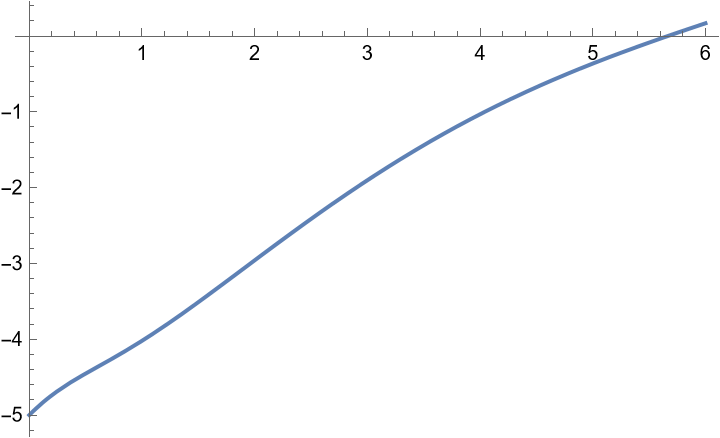
\includegraphics[scale=0.8]{pic_1.png}$$
	Функция $g(x) \in C^{(1)}[0,6]$, то есть она непрерывно дифференцируема на рассматриваемом отрезке. Следовательно, возьмем производную $$g'(x) = 1 + \dfrac{1}{2}\cos\dfrac{x}{2} + \dfrac{1-x^2}{(1+x^2)^2}.$$
	Сделаем грубую оценку этой производной. Функция $g'(x)$ убывает на отрезке $[0,6]$. Поэтому оценим производную по значениям на крайних точках отрезка следующим образом: $g(0)= 2.5$, $g(6)\approx 0.48$, тогда $$0.4\leq g'(x) \leq 2.5.$$
	Таким образом, мы получили значения $$k_1 = 0.4,\quad k_2 = 2.5.$$
	Перепишем исходное уравнение в виде $x =x - \lambda g(x) = f(x)$.
	Причем в качестве $\lambda$ возьмем значение $$\lambda = \dfrac{2}{k_1 + k_2} = \dfrac{2}{0.4 + 2.5} \approx 0.6897.$$
	То есть с помощью ограничений мы выбрали параметр $\lambda$ таким образом, чтобы полученное отображение было сжимающим:
	$$x = \underbrace{x - 0.6897 \cdot (x + \sin\dfrac{x}{2}+\dfrac{x}{1+x^2} - 6)}_{f(x)}.$$
	Для производной можно воспользоваться оценкой
	$$|f'(x)| \leq \dfrac{k_2-k_1}{k_2 + k_1}  = \dfrac{2.5 -0.4}{2.5 + 0.4}\approx 0.7241.$$ 
	Это значение мы можем использовать в качестве коэффициента сжатия, т.е. $$\alpha = 0.7241.$$
	Мы получили отображение $f$, которое будет являться сжимающим, и вычислили для него коэффициент сжатия. Тогда по теореме полученное уравнение $x = f(x)$ имеет единственное решение $x^*\in[a,b]$, которое может быть найдено методом последовательных приближений $$x_n = x_{n-1} - 0.6897 \cdot \Big(x_{n-1} + \sin\dfrac{x_{n-1}}{2}+\dfrac{x_{n-1}}{1+x_{n-1}^2} - 6\Big),\ n=1,2,\ldots$$
	Итерационный процесс метода последовательных приближений мы будем заканчивать при выполнении неравенства (из апостериорной оценки точности):
	$$\dfrac{\alpha}{1 - \alpha}\Norm{x_n - x_{n+1}} \leq \epsilon.$$ 
	Априорное число итераций мы вычислим по формуле (из априорной оценки точности) $$n_{apr} = \Big[\log_\alpha \dfrac{\epsilon(1-\alpha)}{\Norm{x_0 - x_1}}\Big] + 1.$$
	Выберем в качестве начального приближения $$x_0 = 5.5.$$
	Листинг программы на Python:
	\begin{python}
		import numpy as np
		import math
		
		def f(x_n):
			return x_n - 0.68965517 * (x_n + math.sin(x_n / 2) + x_n / (1 + x_n**2)  - 6)
		
		def apriori(x_0, x_1, epsilon, alpha):
			return math.floor(math.log(epsilon * (1 - alpha) / (abs(x_0 - x_1)), alpha)) + 1
		
		def aposteriori(x_n, x_n1, alpha):
			return alpha / (1 - alpha) * abs(x_n - x_n1)
		
		def msa(x_0, x_1, alpha, epsilon):
			iterations = 0
			while True:
			iterations += 1
			x_0 = x_1
			x_1 = f(x_0)
			if aposteriori(x_1, x_0, alpha) <= epsilon:
				break
			return x_1, iterations
		
		x_0 = 5.50
		alpha = 0.72413793
		epsilon = 1e-4
		
		n_apr = apriori(x_0, f(x_0), epsilon, alpha)
		print('apriori number of iterations: ' + str(n_apr))
		
		last_iteration, iterations = msa(x_0, f(x_0), alpha, epsilon)
		print('aposteriori number of iterations: ' + str(iterations))
		print('solution: ' + str(last_iteration))\end{python}
	Результат вывода:\\\\
	apriori number of iterations: 23\\
	aposteriori number of iterations: 16\\
	solution: 5.387649268435892\\\\
	Таким образом, мы получили следующие значения:
	\begin{itemize}
		\item априорное (предполагаемое) число итераций равно 23;
		\item апостериорное (реальное) число итераций равно 16;
		\item приближенное решение исходного уравнения равно $$x^* \approx 5.3876$$
	\end{itemize}
	\section*{ПРИМЕНЕНИЕ ПРИНЦИПА СЖИМАЮЩИХ ОТОБРАЖЕНИЙ ДЛЯ РЕШЕНИЯ СЛАУ}
	Пусть дана система линейных алгебраических уравнений вида
	$$
	\begin{cases}
		a_{11} x_{1}+a_{12} x_{2}+\ldots+a_{1 m} x_{m}=b_{1}, \\
		a_{21} x_{1}+a_{22} x_{2}+\ldots+a_{2 m} x_{m}=b_{2}, \\
		\dotfill\\
		a_{m 1} x_{1}+a_{m 2} x_{2}+\ldots+a_{m m} x_{m}=b_{m},
	\end{cases}\eqno(1)
	$$
	которую можно записать в матричном виде
	$$
	A X=B\eqno(2)
	$$
	Предположим, что определитель $\operatorname{det} A \neq 0$, тогда существует единственное решение системы $(1)$. Для применения принципа сжимающих отображений перепишем уравнение $(2)$ в виде
	$$
	X=C X+D\eqno(3)
	$$
	Обозначим через $F(X)=C X+D$, тогда отображение $F: \mathbb{R}^{m} \rightarrow \mathbb{R}^{m}$ задается системой линейных уравнений $$
	y_{i}=\sum_{j=1}^{m} c_{i j} x_{j}+d_{i}(i=1,2, \ldots, m)
	$$
	Если отображение $F$ --- сжатие, то мы можем применить метод последовательных приближений к решению уравнения $X=F(X)$.
	\begin{theorem}
		Если матрица C системы $(3)$ такова, что $0 \leqslant \alpha<1$, где величина $\alpha$ определяется формулой $$
		\alpha=\max _{1 \leqslant i \leqslant m} \sum_{j=1}^{m}\left|c_{i j}\right|<1
		$$
		или 
		$$
		\alpha=\max _{1 \leqslant j \leqslant m} \sum_{i=1}^{m}\left|c_{i j}\right|<1,
		$$ то система уравнений $(3)$ имеет единственное решение. Это решение может быть найдено методом последовательных приближений
		$$
		x_{i}^{(n+1)}=\sum_{j=1}^{m} c_{i j} x_{j}^{(n)}+d_{i}
		$$
		а в качестве $x^{(0)}=\left(x_{1}^{(0)}, \ldots, x_{m}^{(0)}\right)$ можно взять любую точку из $\mathbb{R}^{m}$. Скорость сходимости итерационного процесса оценивается неравенством $$\Norm{x_n-x^*} \leq \dfrac{\alpha^n}{1-\alpha}\Norm{x_0-x_1}.$$
	\end{theorem}
	Важно заметить, что если матрица $C=\left(c_{i j}\right)_{i, j=1}^{m}$ симметрична, то по сферической норме условие сжатия имеет вид
	$$
	\sum_{j=1}^{m} \sum_{i=1}^{m}\left|a_{i j}\right|<1
	$$
	и, фактически означает, что $\|C\|<1$. Из курса линейной алгебры известно, что $\|C\|$ совпадает с $\left|\lambda_{1}\right|$, где $\lambda_{1}$ --- наибольшее по абсолютной величине собственное значение матрицы $C$. Тогда условие сжатия не только достаточно, но и необходимо для сходимости метода последовательных приближений.\\\\
	Таким образом, когда матрица $C$ симметрична, процесс последовательных приближений для решения системы линейных уравнений сходится к решению тогда и только тогда, когда все собственные значения матрицы $C$ меньше единицы по абсолютной величине.\\\\
	Обратимся к вопросу преобразования системы $(2)$ к виду $(3)$.
	Самый простой способ следующий. Из первого уравнения $(1)$ выразим $x_{1}$, из второго $x_{2}$ и т. д. Тогда на главной диагонали матрицы $C$ стоят нули, а ненулевые элементы выражаются по формулам
	$$
	c_{i j}=\frac{a_{i j}}{a_{i i}}, d_{i}=\frac{b_{i}}{a_{i i}}, i, j=\overline{1, m},\quad i \neq j
	$$
	Обратимся ко второму способу. Пусть $A^{\top}$ --- транспонированная к $A$ матрица, $E$ --- единичная матрица, $\lambda\left(A^{\top} A\right)$ --- максимальное собственное значение матрицы $A^{\top} A$. Тогда исходное уравнение $(2)$ можно записать так:
	$$
	X=\left(E-\frac{A^{\top} A}{\lambda\left(A^{\top} A\right)}\right) X+\frac{A^{\top} B}{\lambda\left(A^{\top} A\right)}
	$$
	тогда
	$$
	C=E-\frac{A^{\top} A}{\lambda\left(A^{\top} A\right)}, D=\frac{A^{\top} B}{\lambda\left(A^{\top} A\right)}
	$$
	Если матрица $C$ получена таким образом, то все ее собственные числа положительны и меньше единицы.
	\section*{ЗАДАЧА 2}
	Найти решение системы линейных алгебраических уравнений $$\begin{cases}
	6.25x_1 - x_2 + 0.5x_3 = 7.5,\\
	-x_1 + 5x_2 + 2.12x_3 = -8.68,\\
	0.5x_1 + 2.12x_2 + 3.6x_3 = -0.24
	\end{cases}$$ с точностью $\epsilon=10^{-4}$. Составить алгоритм и написать программный код, реализующий метод последовательных приближений, предусматривающий:
	\begin{itemize}
		\item приведение системы к специальному виду для применения метода последовательных приближений;
		\item вычисление коэффициента сжатия;
		\item вычисление априорной оценки количества итераций;
		\item вывод на печать последней итерации и ее номера.
	\end{itemize}
	Данную нам систему перепишем в матричном виде $$AX = B,$$ где $$A = \begin{pmatrix}
	6.25 & -1 & 0.5\\
	-1 & 5 & 2.12\\
	0.5 & 2.12 & 3.6
	\end{pmatrix},\quad B = \begin{pmatrix}
	7.5 \\ -8.68 \\ -0.24
	\end{pmatrix}.$$
	Можно легко проверить, что $\det A \approx -77.44 \ne 0$, то есть матрица $A$ невырождена. Значит для данной системы существует единственное решение. Чтобы применить принцип сжимающих отображений, перепишем уравнение в виде $$X = \underbrace{CX + D}_{F(X)}.$$
	Следующим шагом будем построение матрицы $C$ и вектора $D$ таких, чтобы мы могли применить принцип сжимающих отображений. Для этого воспользуемся формулой $$
	C=E-\frac{A^{\top} A}{\lambda\left(A^{\top} A\right)}, D=\frac{A^{\top} B}{\lambda\left(A^{\top} A\right)}
	$$
	Так как полученная таким образом матрица имеет все собственные значения меньше единицы, то мы сможем воспользоваться методом последовательных приближений для отыскания решения системы.\\\\
	Мы не будем считать вручную матрицу $C$ и $D$, а сразу реализуем алгоритм для вычисления по указанной выше формуле. Сперва вычислим матрицу $C$:
	\begin{python}
		import numpy as np
		import math
		
		A = np.array([
		[6.25, -1, 0.5],
		[-1, 5, 2.12],
		[0.5, 2.12, 3.6]])
		B = np.array([[7.5], [-8.68], [-0.24]])
		
		C = np.eye(A.shape[0]) - (np.dot(A.T, A)) / max(np.linalg.eigvals(np.dot(A.T, A)))
		
		print(*C, sep='\n')\end{python}
	Результат вывода:
	$$[ 0.17960243\quad  0.20737615\quad -0.05708441]$$
	$$[ 0.20737615\quad  0.37941007\quad -0.360863  ]$$
	$$[-0.05708441\quad -0.360863\quad    0.63969869]$$
	Теперь вычислим вектор $D$:
	\begin{python}
		D = (np.dot(A.T, B) / max(np.linalg.eigvals(np.dot(A.T, A))))
		print(*D, sep='\n')\end{python}
	Результат вывода: \begin{center}
		$[1.12815477]$\\
		$[-1.04621778]$\\
		$[-0.31575716]$
	\end{center}
	Таким образом, мы получили матрицу $$C = \begin{pmatrix}
		0.17960243 &  0.20737615 & -0.05708441\\
		0.20737615 &  0.37941007 & -0.360863\\
		-0.05708441 & -0.360863 & 0.63969869
	\end{pmatrix},\quad D = \begin{pmatrix}
	1.12815477\\
	-1.04621778\\
	-0.31575716
	\end{pmatrix}$$
	Матрица $C$ симметрическая. Следовательно, процесс последовательных приближений для решения системы линейных уравнений сходится к решению тогда и только тогда, когда все собственные значения матрицы $C$ меньше единицы по абсолютной величине.
	Вычислим модули собственных чисел матрицы $C$:
	\begin{python}
		print(*abs(np.linalg.eigvals(C)))\end{python}
	Результат вывода:
	\begin{center}
		$0.9309731403755809,\quad 9.628392918029083e-17,\quad 0.2677380489149452$
	\end{center}
	То есть мы можем применить процесс последовательных приближений для отыскания приближенного решения исходной системы в виде $$X_n = F(X_{n-1}) = CX_{n-1} + D.$$
	Итерационный процесс метода последовательных приближений мы будем заканчивать при выполнении неравенства (из апостериорной оценки точности):
	$$\dfrac{\alpha}{1 - \alpha}\Norm{X_n - X_{n+1}} \leq \epsilon.$$ 
	Априорное число итераций мы вычислим по формуле (из априорной оценки точности) $$n_{apr} = \Big[\log_\alpha \dfrac{\epsilon(1-\alpha)}{\Norm{X_0 - X_1}}\Big] + 1.$$
	Выберем в качестве начального приближения нулевой вектор $$X_0 = (0,0,0)^T.$$
	В качестве оценки для коэффициента сжатия возьмем $$\alpha = \Norm{C}_2.$$
	Листинг программы на Python:
	\begin{python}
		def F(X_n):
			return np.dot(C, X_n) + D
		
		def aposteriori(X_n, X_n1, alpha):
			return alpha / (1 - alpha) * np.linalg.norm(X_n - X_n1, 2)
		
		def apriori(X_0, X_1, epsilon, alpha):
			return math.floor(math.log(epsilon * (1 - alpha) / (np.linalg.norm(X_0 - X_1, 2)), alpha)) + 1
		
		def msa(X_0, X_1, alpha, epsilon):
			iterations = 0
			while True:
				iterations += 1
				X_0 = X_1
				X_1 = F(X_0)
					if aposteriori(X_1, X_0, alpha) <= epsilon:
						break
			return X_1, iterations
		
		X_0 = np.zeros([3,1])
		alpha = np.linalg.norm(C, 2)
		epsilon = 1e-4
		
		print('compression coefficient: ' + str(alpha))
		
		n_apr = apriori(X_0, F(X_0), epsilon, alpha)
		print('apriori number of iterations: ' + str(n_apr))
		
		last_iteration, iterations = msa(X_0, F(X_0), alpha, epsilon)
		print('aposteriori number of iterations: ' + str(iterations))
		print('solution: \n' + str(last_iteration))\end{python}
		Результат вывода:\\\\
		compression coefficient: 0.9309731403755804\\
		apriori number of iterations: 173\\
		aposteriori number of iterations: 136\\
		solution: 
		\begin{center}
			$[[ 0.80002193]$\\
			$[-1.99994162]$\\
			$[ 0.99992337]]$
		\end{center}
		Таким образом, мы получили следующие значения:\begin{itemize}
			\item коэффициент сжатия равен $\approx 0.931$
			\item априорное число итераций равно 173;
			\item апостериорное число итераций равно 136;
			\item приближенное решение исходной системы равно $$X^* \approx \begin{pmatrix}
			0.8000\\
			-1.9999\\
			0.9999
			\end{pmatrix}.$$ 
		\end{itemize}
		\section*{ПРИМЕНЕНИЕ ПРИНЦИПА СЖИМАЮЩИХ ОТОБРАЖЕНИЙ ДЛЯ РЕШЕНИЯ ИНТЕГРАЛЬНЫХ УРАВНЕНИЙ}
		Интегральными уравнениями называют уравнения относительно неизвестной функции, входящей в уравнение под знаком интеграла.
		\\\\
		Ограничимся рассмотрением уравнений вида
		$$
		a(t) x(t)-\int_{a}^{b} \mathcal{K}(t, s ; x(s)) \mathrm{d} s=y(t),\quad t \in[a, b]\eqno(1)
		$$
		здесь $a(t), y(t)$ --- заданные функции; $\mathcal{K}(t, s ; x(s))$ --- заданная функция, называемая \textit{ядром интегрального уравнения}; $x(t)$ --- неизвестная функция. Решение $x(t)$ разыскивается в различных пространствах функций в зависимости от свойств функции $\mathcal{K}(t, s ; z)$ и $y$. Пространства выбираются так, чтобы интеграл в (1) существовал. Уравнение (1) называется уравнением Фредгольма. Если $a(t) \equiv 0$, то уравнение (1) называется уравнением Фредгольма первого рода, соответственно, при $a(t) \equiv 1$ --- второго рода и уравнением третьего рода при $a(t) \neq 0$. Исследование уравнений второго и третьего рода не отличаются, поэтому мы ограничимся рассмотрением случая $a(t)=1$.
		\\\\
		Интегральное уравнение (1) называется линейным, если функция $\mathcal{K}(t, s, z)$ линейна по $z$. Если $y(t)=0$, то уравнение (1) называется однородным, в противном случае неоднородным.
		\\\\
		Решением уравнения (1) называется функция $x(t)$, при подстановке которой в уравнение выполняется равенство для всех $t \in[a, b]$ или почти всех. Линейное однородное уравнение всегда имеет решение $x(t) \equiv 0$.
		\\\\
		Выделим класс уравнений с переменным верхним пределом вида
		$$
		a(t) x(t)-\int_{a}^{t} \mathcal{K}(t, s ; x(s)) \mathrm{d} s=y(t)
		$$
		называемые интегральными уравнениями Вольтерра.
		\\\\
		Уравнение Вольтерра является частным случаем уравнения Фредгольма, если переопределить ядро $\mathcal{K}(t, s ; x(s))$.\\\\
		Идея применения принципа сжимающих отображений и интегральным уравнениям (29) либо (30) заключается в следующем.
		\\\\
		Пусть имеется интегральное уравнение
		$$
		x(t)=\int_{T} \mathcal{K}(t, s ; x(s)) \mathrm{d} s+y(t)
		$$
		где $T=[a, b]$ либо $T=[a, t]$. Соответствие $x \rightarrow \int_{T} \mathcal{K}(t, s ; x(s)) \mathrm{d} s+y(t)$ определяет отображение множества функций, заданных на $T$, на себя. Тогда уравнение (31) записывается в виде $x=F(x)$, а это означает, что искомое решение является неподвижной точкой отображения $F$. Для того, чтобы применить принцип сжимающих отображений, нужно\begin{itemize}
			\item выбрать банахово пространство функций;
			\item проверить, что (31) определяет сжимающее отображение.
		\end{itemize}
		Покажем, каким образом такая схема реализуется в пространстве $C[a, b]$ непрерывных функций на отрезке $[a, b]$ для линейного неоднородного уравнения Фредгольма
		$$
		x(t)-\lambda \int_{a}^{b} \mathcal{K}(t, s) x(s) \mathrm{d} s=y(t)
		$$
		\begin{theorem}
			 Пусть $\mathcal{K}(t, s)$ - непрерывная функиия на множестве $[a, b] \times[a, b]=\Omega$ и $M=\max _{(t, s) \in \Omega}|\mathcal{K}(t, s)|$, тогда для любого $\lambda$ такого, что $|\lambda|<\frac{1}{M(b-a)}$ интегральное уравнение Фредгольма второго рода имеет единственное решение для любой правой части $y(t) \in C[a, b]$. 
		\end{theorem}
		На практике при численной реализации метода последовательных приближений необходимо приближенно вычислять интегралы по методу квадратур, что вносит дополнительную погрешность и довольно большую при большом числе итераций. С этой целью интегрирование нужно выполнять с большей точностью, чем погрешность метода последовательных приближений.\\\\
		Так, для приближенного вычисления интеграла от гладкой функции хорошо подходит метод Симпсона или метод парабол.
		$$\int_{a}^{b} f(t) \mathrm{d} t \approx \frac{b-a}{m}\left[f_{0}+f_{m}+2\left(f_{2}+f_{4}+\ldots+f_{m-2}\right)+4\left(f_{1}+f_{3}+\ldots+f_{m-1}\right)\right],$$ где $f_{m}=f\left(t_{m}\right), t_{m}=t_{0}+\frac{b-a}{m}$.\\\\
		Обозначим через $t_{i}, i=0,1, \ldots, m$ узлы сетки, расположенной на отрезке $a, b$. Тогда соотношение (33) перепишется в виде
		$$
		x_{n}\left(t_{i}\right)=\lambda \int_{a}^{b} \mathcal{K}\left(t_{i}, s\right) x_{n-1}\left(s_{i}\right) \mathrm{d} s+y\left(t_{i}\right)
		$$
		Если воспользоваться квадратурной формулой трапеций на равномерной сетке с шагом $h=\frac{b-a}{m}$, то расчетные формулы метода последовательных приближений примут вид
		$$
		\begin{gathered}
			x_{n}\left(t_{i}\right)=\lambda \frac{h}{2}\left[k_{i, 0} x_{n-1,0}+2\left(k_{i, 1} x_{n-1,1}+\ldots k_{i, m-1} x_{n-1, m-1}\right)+k_{i, m} x_{n-1, m}\right]+ \\
			+y\left(t_{i}\right), i=0,1, \ldots, m .
		\end{gathered}
		$$
		Здесь $k_{i, j}=\mathcal{K}\left(t_{i}, s_{j}\right), x_{n, j}=x_{n}\left(s_{j}\right)$.
		\\\\
		Отметим, что при решении линейных интегральных уравнений сходимость метода последовательных приближений не зависит от вида правой части и начального приближения, которые влияют на скорость сходимости итерационного процесса.
		\\\\
		Разрешимость уравнений Фредгольма зависит от условий на ядро. Покажем, что для уравнения Вольтерра условие разрешимости проще.\\\\
		Рассмотрим линейное неоднородное уравнение Вольтерра
		$$
		x(t)-\lambda \int_{a}^{t} \mathcal{K}(t, s) x(s) \mathrm{d} s=y(t) .
		$$
		Выясним, когда можно применить метод последовательных приближений для его решения.
		\begin{theorem}
			Пусть $\mathcal{K}(t, s)$ --- непрерывная функция по переменным $t$ и $s$. Тогда для любой $y(t) \in C[a, b]$ и любого $\lambda$ из поля $P$ интегральное уравнение Вольтерра второго рода имеет единственное решение.
		\end{theorem}
		\section*{ЗАДАЧА 3}
		Выяснить, при каких значениях параметра $\lambda \ne 0$ к интегральному уравнению Фредгольма второго рода
		$$
		x(t) - \lambda\int\limits_0^1e^{t-s} x(s)\mathrm{d} s = 1
		$$
		применим принцип сжимающих отображений в пространстве $C[0,1]$ и в пространстве $L_2[0,1]$. При $\lambda = \lambda_0$ найти приближенное решение уравнения с точностью $\epsilon = 10^{-3}$ и сравнить его с точным решением. Составить алгоритм и написать программный код, реализующий метод последовательных приближений, предусматривающий:
		\begin{itemize}
			\item приведение интегрального уравнения к специальному виду для применения метода последовательных приближений;
			\item вычисление коэффициента сжатия;
			\item вычисление априорной оценки количества итераций;
			\item выбор начального приближения;
			\item составление итерационного процесса в каждой фиксированной точке $t_i$, $i=1,\ldots, n$ по правилу $$x_{n}\left(t_{i}\right)=\lambda \int_{a}^{b} \mathcal{K}\left(t_{i}, s\right) x_{n-1}\left(s\right) \mathrm{d} s+y\left(t_{i}\right)$$
			с приближенным вычислением интеграла по формуле Симсона с шагом $0.05$;
			\item вывода на печать номера последней итерации, апостериорной погрешности, графика точного и приближенного решения.
		\end{itemize}
		Исходное уравнение представляет собой интегральное уравнение с вырожденным ядром, поэтому мы можем найти его точное решение. Перепишем уравнение в виде $$x(t) =\lambda e^t\int\limits_0^1e^{-s} x(s)\mathrm{d} s +1.$$
		Обозначим $$c = \int\limits_0^1e^{-s} x(s)\mathrm{d} s. $$
		Тогда $$x(t) = \lambda e^t c + 1.$$
		Подставим это выражение в предыдущее уравнение и получим $$c = \int\limits_0^1e^{-s}(\lambda e^s c + 1)\mathrm{d} s = \lambda c s\Big|_0^1 - e^{-s}\Big|_0^1 = \lambda c - e^{-1} + 1.$$
		Отсюда $$c = \dfrac{1 - e^{-1}}{\lambda - 1}.$$
		Тогда точное решение исходного интегрального имеет вид $$x(t) = \lambda \dfrac{e^t - e^{t-1}}{\lambda - 1} + 1.$$
		Теперь попробуем вычислить приближенное решение для данного интегрального уравнения.
		Приведем исходное интегральное уравнение к виду $$x = F(x),$$ тогда мы сможем применить принцип сжимающих отображений, если в рассматриваемых банаховых пространствах отображение является сжимающим. Таким образом, исходное уравнение примет вид $$x(t) =\underbrace{ \lambda\int\limits_0^1e^{t-s} x(s)\mathrm{d} s +1}_{F(x)}.$$
		\subsection*{ПРОСТРАНСТВО $C[0,1]$}
		В пространстве $C[0,1]$ отображение $F:C[0,1] \to C[0,1]$, так как представляет собой сумму непрерывных функций. Покажем, что отображение $F$ является сжимающим. Для этого покажем выполнение условия: $\exists \alpha \in \mathbb{R},\ 0<\alpha<1:$ $$\Norm{F(x) - F(y)}_{C[0,1]} \leq \alpha\Norm{x - y}_{C[0,1]},\quad \forall x,y \in {C[0,1]}.$$
		Рассмотрим \begin{multline*}
			\Norm{F(x) - F(y)}_{C[0,1]} = \underset{0\leq t \leq 1}{\max} \Big|\lambda \int\limits_0^1e^{t-s} (x(s) - y(s))\mathrm{d} s\Big| \leq\\ \leq |\lambda|e\cdot  \underset{0\leq t \leq 1}{\max} |x(s) - y(s)| \cdot\int\limits_0^1e^{-s} ds = \underbrace{|\lambda| (e-1)}_\alpha \Norm{x - y}_{C[0,1]}.
		\end{multline*}
		Отсюда следует, что $\alpha = |\lambda| (e-1) < 1$. Значит выбираем $\lambda$ такое, что $$|\lambda| < \dfrac{1}{e - 1}\approx 0.582.$$ При таких $\lambda$ можно применять принцип сжимающих отображений. \\\\
		Вычислим априорную оценку количества итераций по формуле $$n_{apr} = \Big[\log_\alpha \dfrac{\epsilon(1-\alpha)}{\Norm{x_0 - x_1}}\Big] + 1.$$
		Пусть $x_0 = 0$, $\lambda = \dfrac{1}{9(e-1)}\approx 0.43$. Тогда коэффициент сжатия равен $\alpha = 0.1111$, а $$x_1 = F(x_0) = 1.$$ Ниже приведен листинг программы, реализующей вычисление коэффициента сжатия с заданными параметрами:
		\begin{python}
			def apriori(x_0, x_1, epsilon, alpha):
				return math.floor(math.log(epsilon * (1 - alpha) / (np.absolute(x_0 - x_1)), alpha)) + 1
			
			lambda_ = 1 / (9*(np.e - 1))
			x_0 = 0
			x_1 = 1
			alpha = np.absolute(lambda_)*(np.e - 1)
			epsilon = 1e-3
			
			n_apr = apriori(x_0, x_1, epsilon, alpha)
			print('apriori number of iterations: ' + str(n_apr))\end{python}
			Результат вывода\\\\
			apriori number of iterations: 4\\\\
			То есть, число $n_{apr} =4.$
			Теперь нам необходимо составить итерационный процесс с приближенным вычислением интеграла по формуле Симсона с шагом $$\dfrac{b-a}{m} = 0.05$$
			Выясним, чему равно $m$ в данной формуле:
			\begin{python}
				a = 0
				b = 1
				step = 0.05
				m = (b-a) / step
				print('m=' + str(m))\end{python} 
				Результат вывода:
				m=20.0\\\\
			Теперь рассчитаем все $t_i$, $i=\overline{1,20}$ узлы сетки, расположенной на $[a,b]$. Выберем $t_0 = 0$ --- левый край отрезка. Далее с шагом $0.05$ будем двигаться, получая остальные $t_i$:
			\begin{python}
				t_i = 0
				grid = [t_i]
				for i in range(int(m)):
					t_i = t_i + (b - a) / m
					grid.append(t_i)\end{python} 
			В результате получили последовательность значений $t_i$ для применения формулы Симсона. Далее реализуем функцию, которая рассчитывает значение интеграла по формуле Симсона $$\int_{0}^{1} f(t) \mathrm{d} t \approx \frac{b-a}{m}\left[f_{0}+f_{m}+2\left(f_{2}+f_{4}+\ldots+f_{m-2}\right)+4\left(f_{1}+f_{3}+\ldots+f_{m-1}\right)\right],$$ где $f_{m}=f\left(t_{m}\right), t_{m}=t_{0}+0.05$. Причем в нашем случае $$f(t) = e^{-t} x_{n-1}(t)$$ и $m=20$.\\\\ Листинг программы:
			\begin{python}
				def simson(a, b, x_n_1):
					step = 0.05
					f = np.exp(-a) * x_n_1[0];
					coord = a
					result = 0
					for i in range(1, m-1):
						if i % 2 == 1:
							result += 4 * np.exp(coord) * x_n_1[i];
						else:
							result += 2 * np.exp(coord) * x_n_1[i];
						coord += step;
					result += np.exp(-b) * x_n_1[m-1];
					result *= step;
					return result;\end{python} 
			Остается реализовать непосредственно итерационный процесс  $$x_{n}\left(t_{i}\right)=\lambda e^{t_i}\int\limits_{0}^{1} e^{-s} x_{n-1}\left(s\right) \mathrm{d} s+1.$$
			Процесс прекращается при выполнении неравенства $$\dfrac{\alpha}{1 - \alpha}\Norm{x_{n-1} - x_{n}} \leq \epsilon.$$
			Причем в нашем случае $x_n = (x_n(t_1), \ldots, x_n(t_m))^T.$ Следовательно возьмем $$\Norm{x_n - x_{n+1}} = \underset{t_i}{\max}|x_{n-1}(t) - x_{n}(t)|.$$
			Листинг программы:
			\begin{python}
				def aposteriori(x_n, x_n1, alpha):
					return alpha / (1 - alpha) * np.linalg.norm(x_n - x_n1, 1)
				
				iterations = 0
				x_n = np.array([0. for _ in range(m + 1)])
				x_n1 = np.array([0. for _ in range(m + 1)])
				
				while True:
					iterations += 1
					for j in range(len(grid)):
						x_n[j] = lambda_ * np.exp(grid[j]) * simson(a, b, x_n1) + 1
					if aposteriori(x_n1, x_n, alpha) <= epsilon:
						break
					x_n1 = np.copy(x_n)\end{python}
			Выведем на печать получившееся число итераций и соответственно шаг сетки, значение приближенного решения и значение точного решения.
			\begin{python}
				def x_actual(t):
					return lambda_ * np.exp(t) * (1 - np.e**(-1)) / (lambda_ - 1) + 1
				print('iterations=' + str(iterations))
				for i in range(len(grid)):
					print('$t=' + str(round(grid[i], 2)) + '\t\t\quad x[approximate]=' + str(x_n[i]) + '\t\t\quad x[actual]=' + str(x_actual(grid[i])) + '$\\\\')\end{python}
				Результат вывода:\\\\
				iterations=12
				\begin{center}
					$t=0		\quad x[approximate]=1.5333335978188036		\quad x[actual]=0.9562985954824286$\\
					$t=0.05		\quad x[approximate]=1.5606781961131433		\quad x[actual]=0.9540579765596405$\\
					$t=0.1		\quad x[approximate]=1.5894247819419953		\quad x[actual]=0.9517024786481203$\\
					$t=0.15		\quad x[approximate]=1.6196452367433605		\quad x[actual]=0.9492262117761651$\\
					$t=0.2		\quad x[approximate]=1.6514151273953734		\quad x[actual]=0.9466229839867649$\\
					$t=0.25		\quad x[approximate]=1.6848138951728617		\quad x[actual]=0.9438862858544859$\\
					$t=0.3		\quad x[approximate]=1.71992505439191		\quad x[actual]=0.9410092742085144$\\
					$t=0.35		\quad x[approximate]=1.756836401239152		\quad x[actual]=0.9379847550211676$\\
					$t=0.4		\quad x[approximate]=1.7956402333079677		\quad x[actual]=0.9348051654190752$\\
					$t=0.45		\quad x[approximate]=1.8364335803905427		\quad x[actual]=0.9314625547720576$\\
					$t=0.5		\quad x[approximate]=1.879318447102889		\quad x[actual]=0.9279485648124093$\\
					$t=0.55		\quad x[approximate]=1.9244020679495168		\quad x[actual]=0.9242544087348755$\\
					$t=0.6		\quad x[approximate]=1.9717971754655528		\quad x[actual]=0.9203708492250624$\\
					$t=0.65		\quad x[approximate]=2.021622282106795		\quad x[actual]=0.9162881753613396$\\
					$t=0.7		\quad x[approximate]=2.0740019765925863		\quad x[actual]=0.911996178332478$\\
					$t=0.75		\quad x[approximate]=2.129067235442505		\quad x[actual]=0.907484125910304$\\
					$t=0.8		\quad x[approximate]=2.1869557504858887		\quad x[actual]=0.9027407356135392$\\
					$t=0.85		\quad x[approximate]=2.2478122731631265		\quad x[actual]=0.8977541464957197$\\
					$t=0.9		\quad x[approximate]=2.3117889764796593		\quad x[actual]=0.8925118894866529$\\
					$t=0.95		\quad x[approximate]=2.3790458355177533		\quad x[actual]=0.8870008562132464$\\
					$t=1.0		\quad x[approximate]=2.4497510274575394		\quad x[actual]=0.8812072662217475$
				\end{center}
			Построим график приближенного и точного решений:
			$$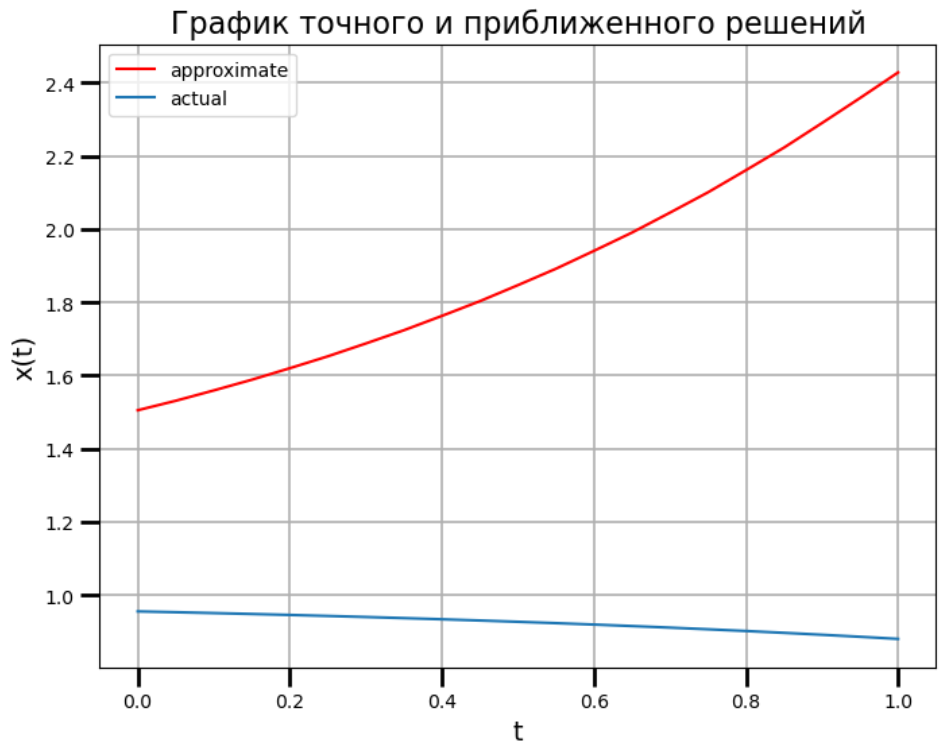
\includegraphics[scale=0.7]{pic_4.png}$$
			\subsection*{ПРОСТРАНСТВО $L_2[0,1]$}
			Рассмотрим пространство $L_2[0,1]$. Покажем, что отображение $F$ является сжимающим. Для этого покажем выполнение условия: $\exists \alpha \in \mathbb{R},\ 0<\alpha<1:$ $$\Norm{F(x) - F(y)}_{L_2[0,1]} \leq \alpha\Norm{x - y}_{L_2[0,1]},\quad \forall x,y \in {L_2[0,1]}.$$
			Сначала запишем в общем виде:
			$$\Big(\int\limits_0^1\Big|\int\limits_0^1 K(t,s) \big(x(s) - y(s)\big)\mathrm{d}s\Big|^2\mathrm{d}t\Big)^\frac12
			\leq \Big(\int\limits_0^1\int\limits_0^1 |K(t,s)|^2 \mathrm{d}s\mathrm{d}t\Big)^\frac12\cdot\underbrace{ \Big(\int\limits_0^1\int\limits_0^1 |x(s) - y(s)|^2 \mathrm{d}s\mathrm{d}t\Big)^\frac12}_{\Norm{x-y}}$$
			Теперь рассмотрим отдельно первый множитель:
			$$\Big(\int\limits_0^1\int\limits_0^1 |K(t,s)|^2 \mathrm{d}s\mathrm{d}t\Big)^\frac12 = |\lambda|\cdot \Big(\int\limits_0^1\int\limits_0^1 e^{2t-2s} \mathrm{d}s\mathrm{d}t\Big)^\frac12 = |\lambda|\cdot \Big(\dfrac{(e - e^{-1})^2}{4}\Big)^\frac12 = |\lambda|\cdot\dfrac{e - e^{-1}}{2} = \alpha.$$
			Следовательно, отображение $F$ отображает пространство $L_2[0,1]$ на себя и является сжимающим, если $$|\lambda| < \dfrac{2}{e + e^{-1}}\approx 0.851$$
			Таким образом, в данном пространстве у нас множество допустимых значений параметра $\lambda$ шире. Соответственно мы можем выбрать $$\lambda = \dfrac{1}{9(e-1)}$$ и так же применить принцип сжимающих отображений. Но теперь изменится априорное число итераций. Снова возьмем начальное приближение $x_0 = 0$. Тогда $$x_1 = F(x_0) = 1.$$
			Отсюда $$\Big(\int\limits_0^1|x_1 - x_0|^2ds\Big)^\frac12 = 1.$$
			Тогда априорное число итераций вычисляем по формуле $$n_{apr} = \Big[\log_\alpha \epsilon(1-\alpha)\Big] + 1.$$
			Листинг программы:
			\begin{python}
				def apriori_L2(epsilon, alpha):
					return math.floor(math.log(epsilon * (1 - alpha), alpha)) + 1
				
				lambda_ = 1 / (9*(np.e - 1))
				alpha = np.absolute(lambda_)*(np.e**2 - 1) / (2*np.e)
				epsilon = 1e-3
				
				n_apr_L2 = apriori_L2(epsilon, alpha)
				print('apriori number of iterations: ' + str(n_apr_L2))\end{python}
				Результат вывода:\\\\
				apriori number of iterations: 3\\\\
				Таким образом, априорное число итераций при одинаковом выборе параметра $\lambda$ в пространстве $L_2[0,1]$ меньше чем в пространстве $C[0,1]$. Однако реальное число итераций останется неизменным так же, как и результаты вычислений. Соответственно все полученные итерации и график мы можем перенести из пространства $C[0,1]$ в пространство $L_2[0,1]$.
		\section*{ЗАДАЧА 4}
		Методом последовательных приближений найти решение интегрального уравнения Вольтерра второго рода в пространстве $C[0,1]$
		$$x(t) + \int\limits_0^t (t-s)x(s)\dif s = 1.$$
		В данном случае ядро $K(t,s) = (t-s)$ является непрерывной функцией по $t$ и $s$. Следовательно уравнение имеет единственное решение. А соответственно применим метод последовательных приближений для отыскания решения данного уравнения.\\\\
		Приведем уравнение к виду $x = F(x)$. Для этого перенесем интеграл из левой части уравнения в правую часть. Тогда $$x(t) = 1-\int\limits_0^t (t-s)x(s)\dif s.$$
		Выберем начальное приближение $x_0(t) = 0$. Тогда $$x_1(t) = 1,$$
		$$x_2(t) = 1-\int\limits_0^t (t-s)\dif s = 1 - \dfrac{t^2}{2},$$
		$$x_3(t) = 1-\int\limits_0^t (t-s)\Big(1 - \dfrac{s^2}{2}\Big)\dif s = 1 - \dfrac{t^2}{2} + \dfrac{t^4}{24},$$
		$$x_3(t) = 1-\int\limits_0^t (t-s)\Big(1 - \dfrac{s^2}{2} + \dfrac{s^4}{24}\Big)\dif s = 1 - \dfrac{t^2}{2} + \dfrac{t^4}{24} - \dfrac{t^6}{720},$$
		$$x_4(t) = 1-\int\limits_0^t (t-s)\Big(1 - \dfrac{s^2}{2} + \dfrac{s^4}{24} - \dfrac{s^6}{720}\Big)\dif s = 1 - \dfrac{t^2}{2} + \dfrac{t^4}{24} - \dfrac{t^6}{720} + \dfrac{t^8}{40320}$$
		и так далее. Получаем, что $$x_n(t) = 1 - \dfrac{t^2}{2!} + \dfrac{t^4}{4!} - \dfrac{t^6}{6!} + \dfrac{t^8}{8!} + \ldots + (-1)^n\dfrac{t^{2n}}{(2n)!}.$$
		Тогда решение интегрального уравнения $$x(t) = \lim\limits_{n\to\infty} x_n(t) = \cos t.$$
		То есть функция $x(t) = \cos t$ и будет являться решением исходного интегрального уравнения, полученным методом последовательных приближений.
\end{document}